\newpage

\section{Projekt platformy}

\subsection{Wprowadzenie}

Jak już wskazałem w poprzednim rozdziale, web scraping odkrywa szczególną rolę w branży e-commerce.
Potwierdza to fakt, że sklepy internetowe stanowią najczęstszy kontekst i przykład ilustrujący to zagadnienie.
Nie inaczej jest w przypadku niniejszej pracy.
W tym rozdziale omówię projekt platformy oraz narzędzia, które składają się na kompletne środowisko sklepu internetowego \href{https://store.tulski.com}{tulski store}.

\subsection{Klaster Kubernetes}

Platformą wdrożeniową dla serwisu jest klaster Kubernetes\cite{what-is-kubernetes}, składający się z czterech węzłów uruchomionych w chmurze obliczeniowej Oracle Cloud Infrastructure.
Każdy węzeł posiada 1 procesor (OCPU) oraz 6 GB pamięci RAM. Większa liczba węzłów pozwala naszemu rozwiązaniowi na wysoką dostępność (ang\. high availability).
W przypadku awarii lub zakłóceń na jednym z węzłów, pozostałe przejmują jego obowiązki, tym samym zapewniając minimalizację przestojów w działaniu aplikacji.

Warto dodać, że cała przedstawiona infrastruktura działa w ramach planu Always Free.
Kolejne podrozdziały mogą stanowić instrukcję stworzenia darmowego klastra Kubernetes dla małych projektów o charakterze edukacyjnym.

\subsubsection{Maszyny wirtualne}

Każdy z węzłów został uruchomiony na osobnej maszynie wirtualnej (ang. virtual machine, VM).

\begin{figure}[H]
    \centering
    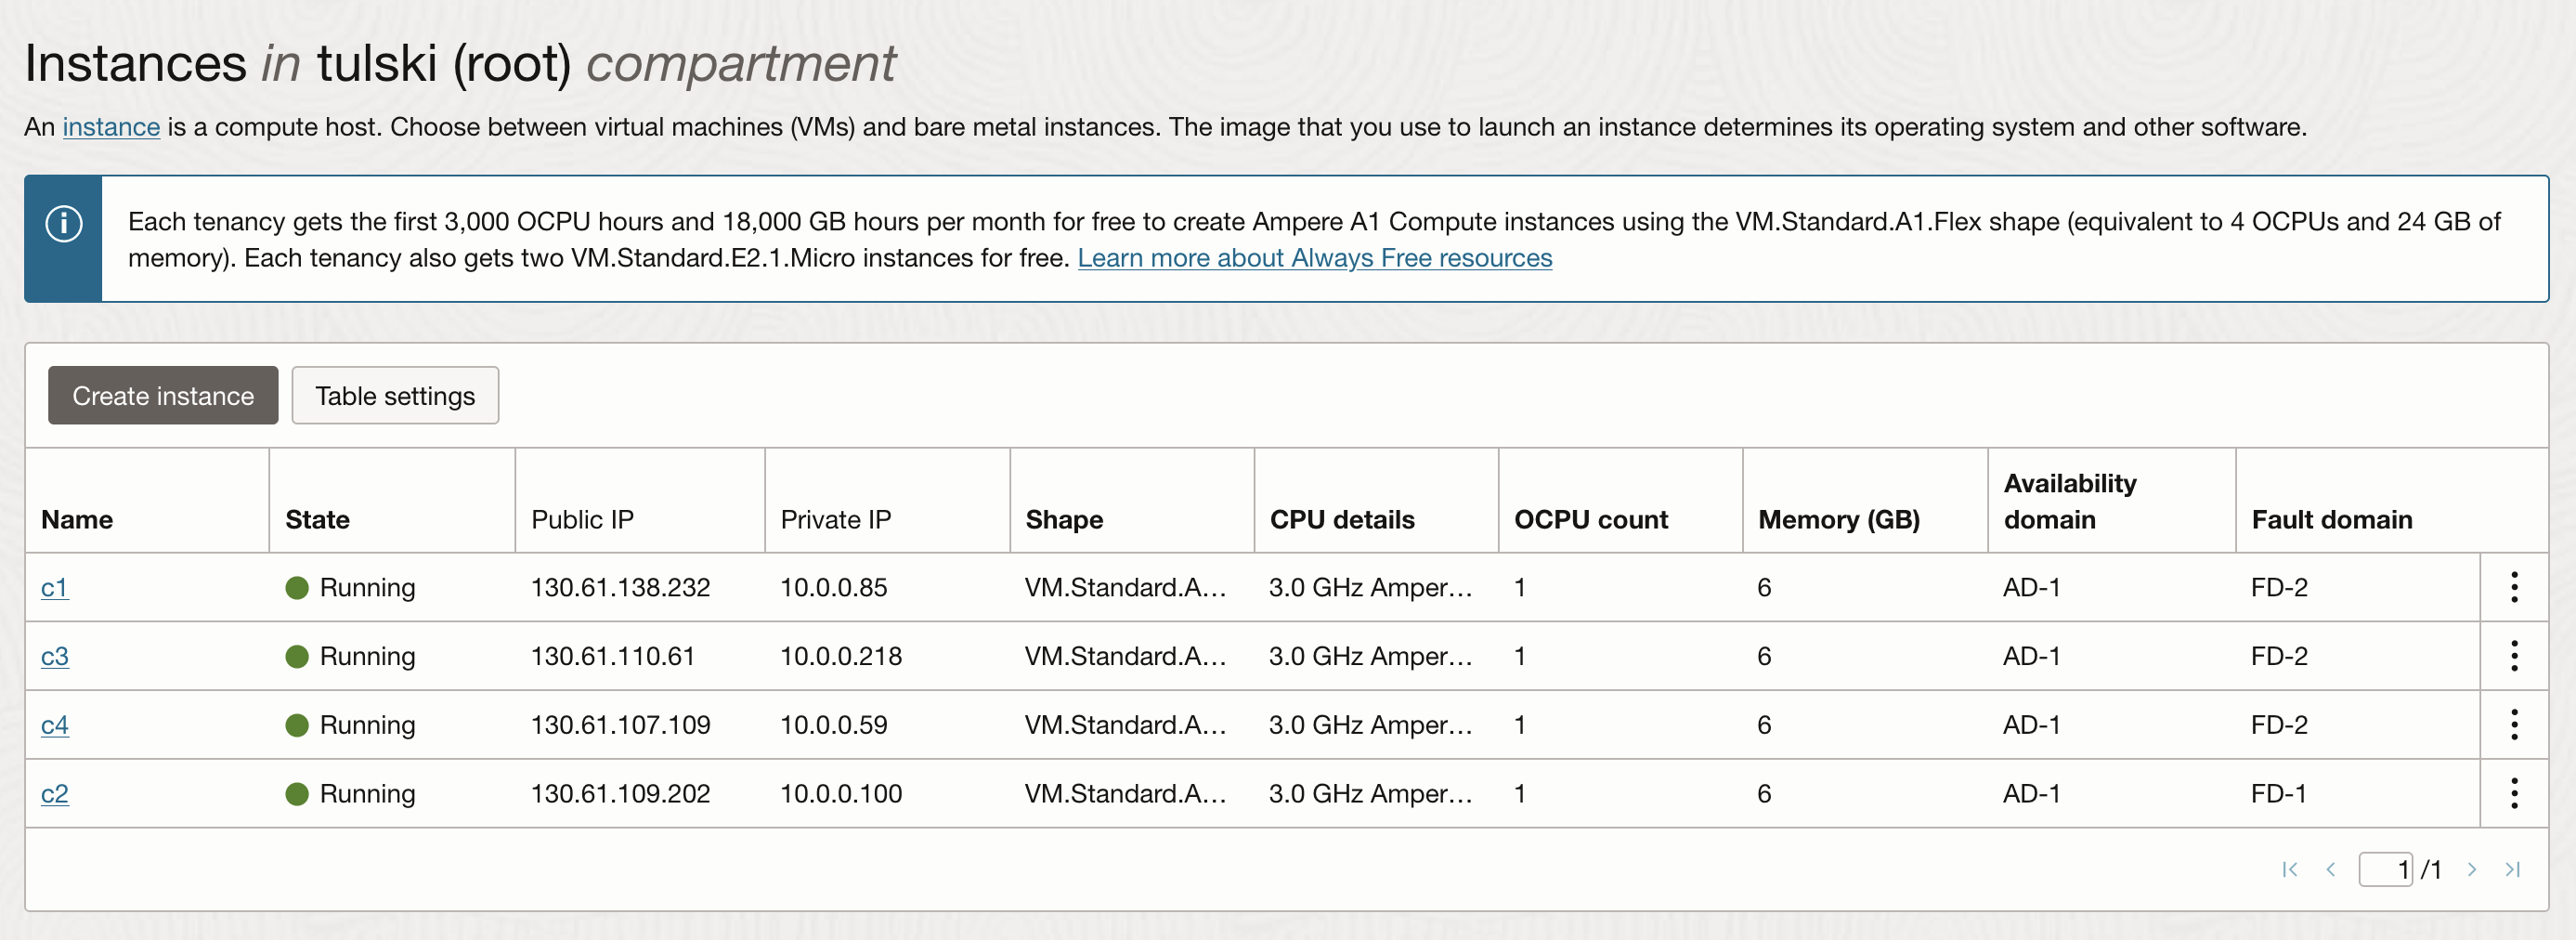
\includegraphics[width=\textwidth]{img/oci-compute-instances}
    \caption{Lista wszystkich maszyn wirtualnych}
    \label{fig:oci-compute-instances}
\end{figure}

\begin{samepage}
    Specyfikacja każdej z maszyn wirtualnych:
    \begin{itemize}
        \item Kształt: VM.Standard.A1.Flex (Procesor Arm od Ampere)
        \item Liczba OCPU: 1
        \item Przepustowość sieci: 1 Gbps
        \item Pamięć RAM: 6 GB
        \item Obraz: Canonical Ubuntu 22.04 aarch64 2023.02.15-0
    \end{itemize}

    \begin{figure}[H]
        \centering
        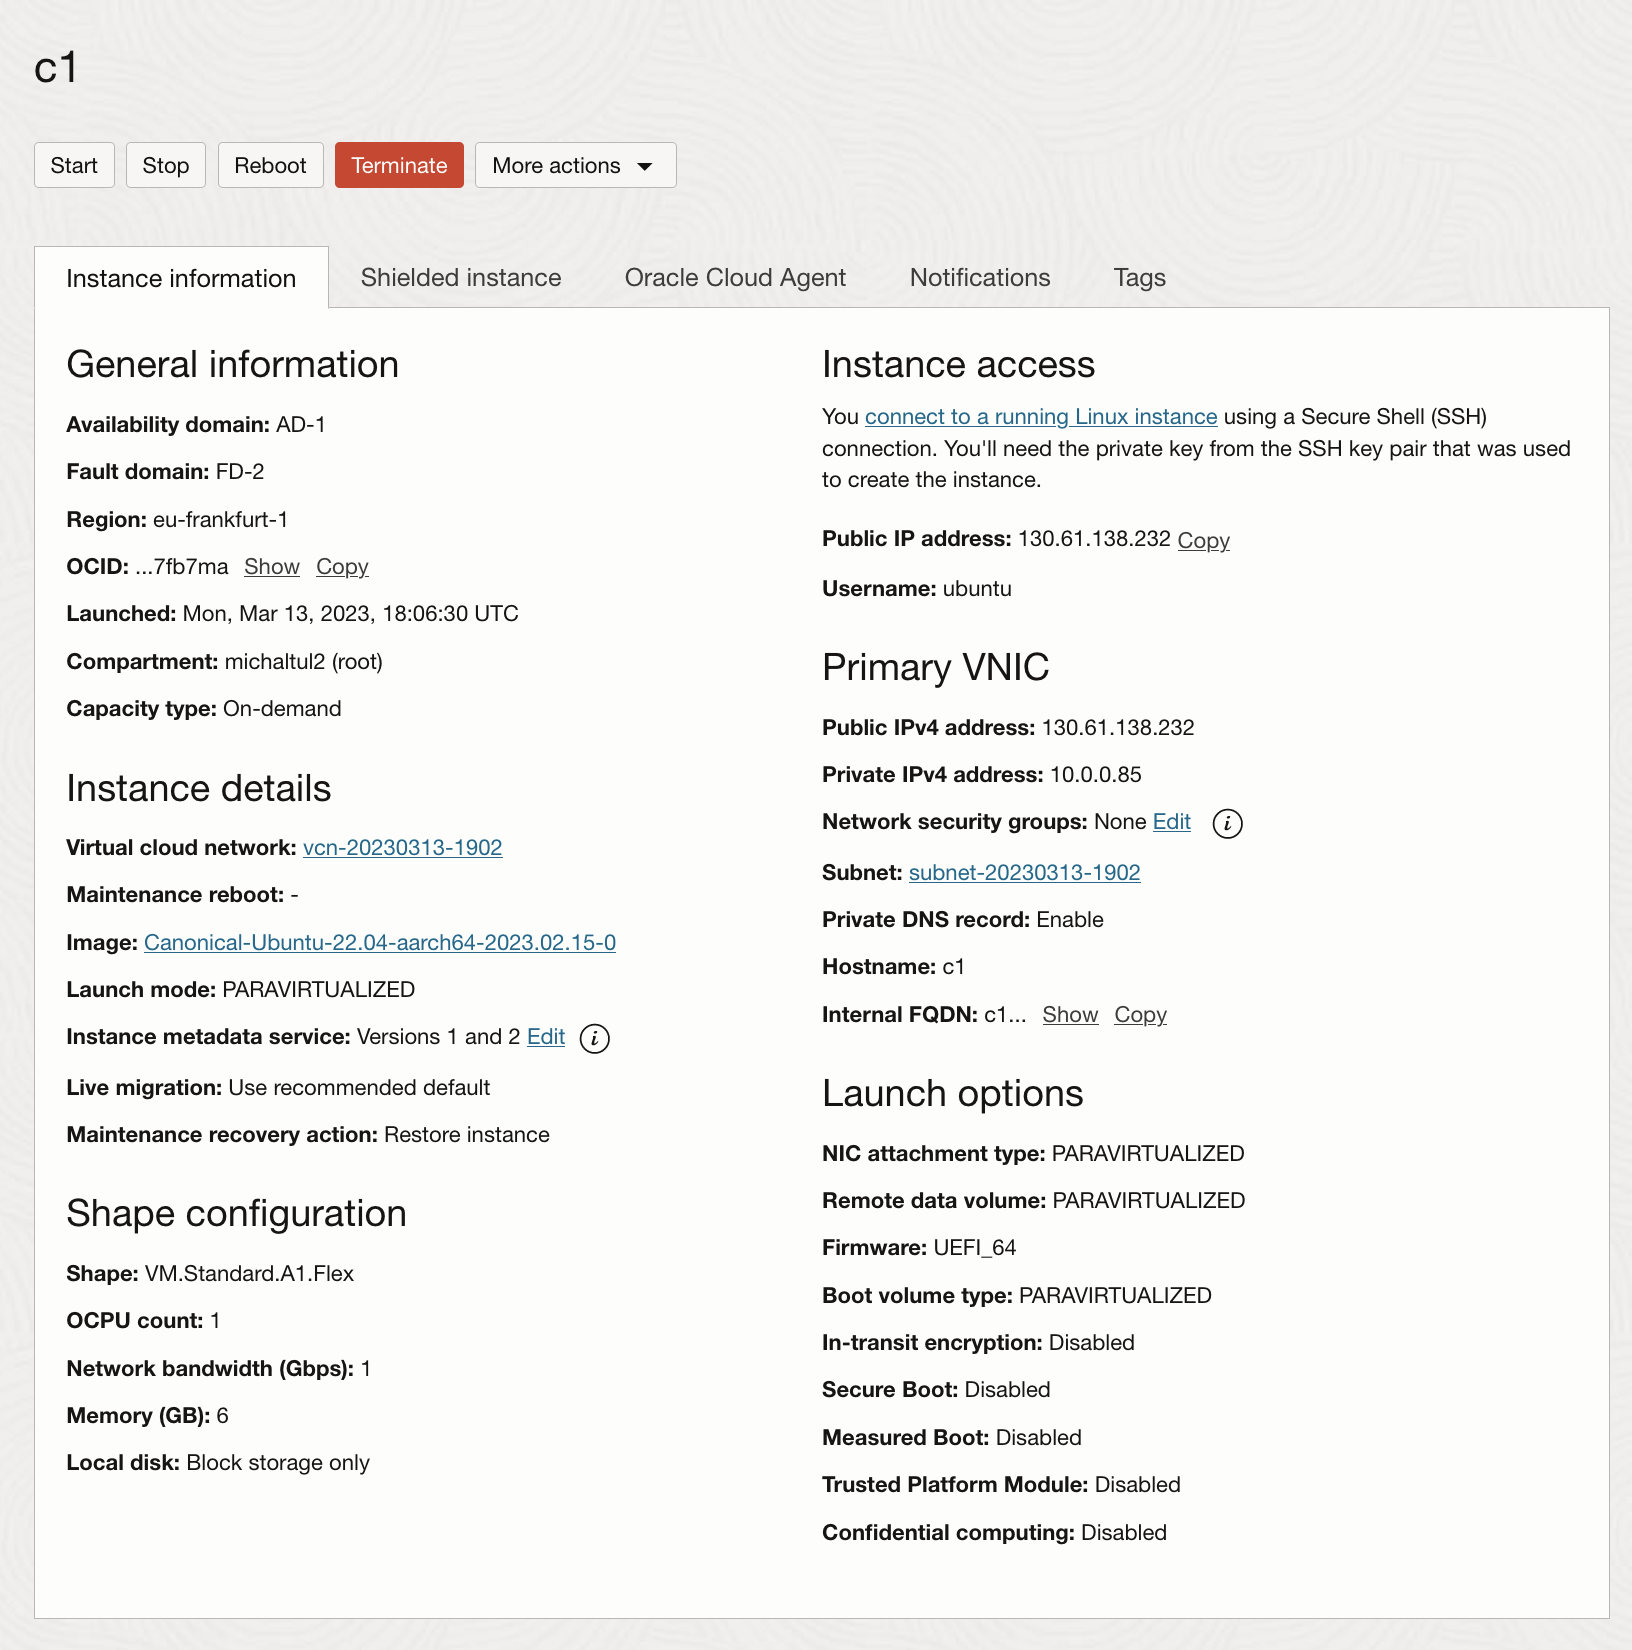
\includegraphics[width=\textwidth]{img/oci-instance-details}
        \caption{Specyfikacja maszyny wirtualnej}
        \label{fig:oci-instance-details}
    \end{figure}
\end{samepage}


\subsubsection{Konfiguracja podsieci}

Wszystkie instancje są połączone w jednej wirtualnej podsieci (ang. virtual cloud network, VCN) subnet-20230313-1902.

\begin{figure}[H]
    \centering
    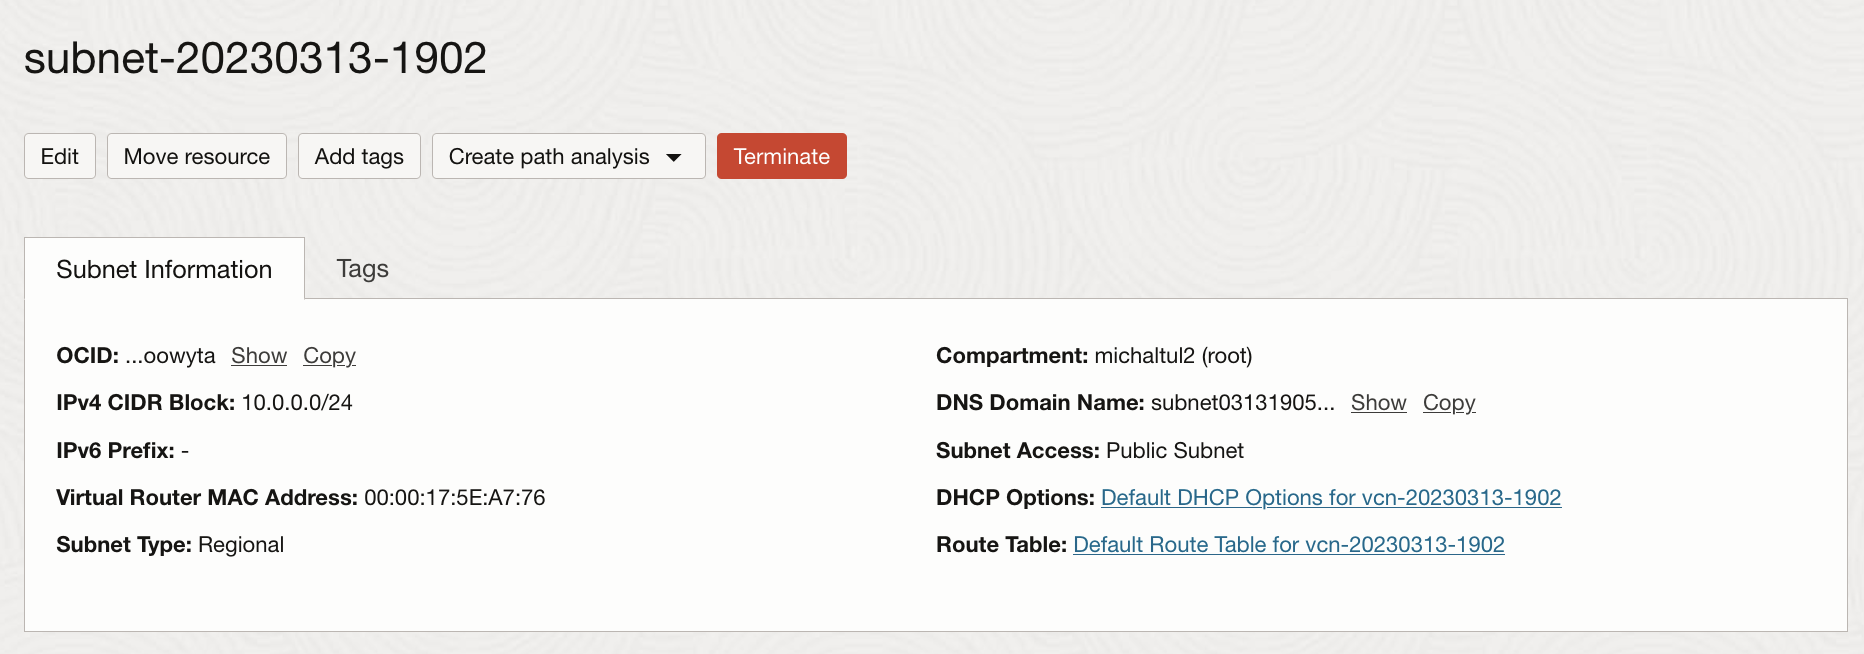
\includegraphics[width=\textwidth]{img/oci-subnet}
    \caption{Podsieć subnet-20230313-1902}
    \label{fig:oci-subnet}
\end{figure}

Domyślne reguły VCN\cite{oci-security-lists} pozwalają na:
\begin{enumerate}
    \item Ruch TCP na porcie usługi SSH (22) z autoryzowanych adresów IP.
    \item Ruch ICMP typu 3 o kodzie 4 (ang. Fragmentation Needed and Don't Fragment was Set) z dowolnego adresu IP.
    \item Ruch ICMP typu 3 z wszystkich hostów znajdujących się w danej podsieci.
    \item Cały ruch wychodzący.
\end{enumerate}

W celu dostosowania reguł do potrzeb projektu zostały dodane dodatkowe dwie reguły.
\begin{enumerate}
    \item Reguła pozwalająca na ruch TCP z dowolnego źródła na porty 80 i 443.
    \item Reguła pozwalająca na cały ruch z adresu IP administratora. Wymagana do zdalnego zarządzania klastrem przez Kubernetes API (kubectl).
\end{enumerate}

\begin{figure}[H]
    \centering
    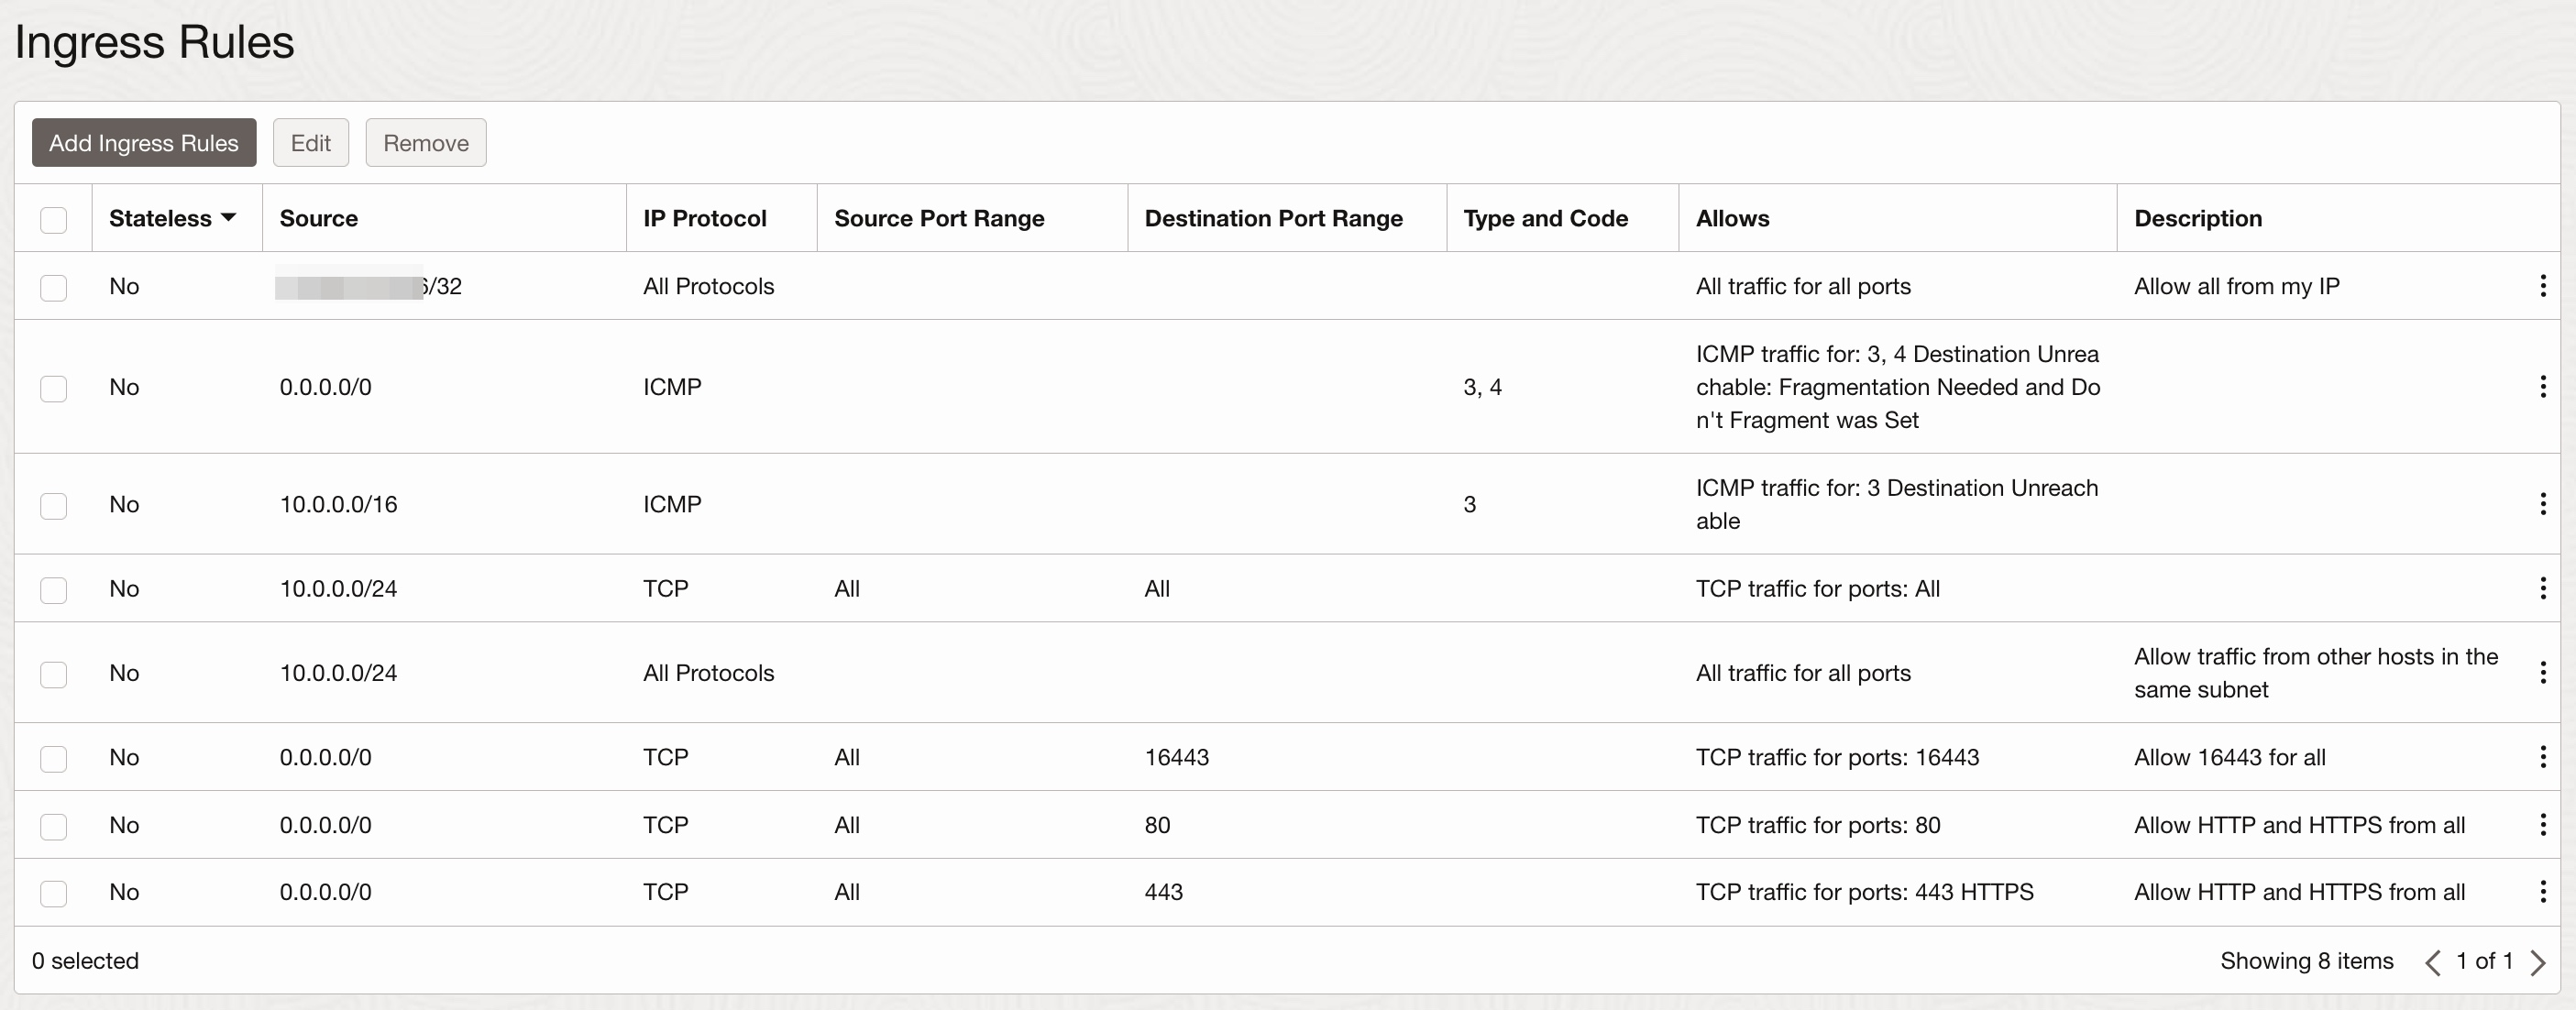
\includegraphics[width=\textwidth]{img/oci-subnet-ingress-rules}
    \caption{Reguły dla ruchu przychodzącego}
    \label{fig:oci-subnet-ingress-rules}
\end{figure}

Zmiany na poziome usług sieciowych OCI są niewystarczające, ponieważ ruch zostanie zablokowany przez domyślne reguły firewalla systemowego maszyn wirtualnych.
Aby zaobserwować oczekiwany rezultat musimy na każdej z maszyn zmodyfikować plik \texttt{/etc/iptables/rules.v4}. Dodajemy dwie reguły:
\begin{enumerate}
    \item Reguła zezwalająca na ruch wejściowy pochodzący z publicznego adresu IP administratora.\\
    \mintinline{text}{-I INPUT -s ADMIN_PUBLIC_IP/32 -j ACCEPT}
    \item Reguła pozwalająca na ruch przychodzący z dowolnego adresu w podsieci.\\
    \mintinline{text}{-I INPUT -s 10.0.0.0/24 -j ACCEPT}
\end{enumerate}

\noindent W dodatku usuwamy wpis, który blokuje wiadomości ICMP (ping):\\
\mintinline{text}{-A FORWARD -j REJECT --reject-with icmp-host-prohibited}

\subsubsection{Network Load Balancer}

Load Balancer (LB) to technologia, która podobnie do reverse proxy ma na celu kierowanie żądań użytkowników do odpowiednich serwerów.
Każdy LB implementuje pewien zestaw reguł i algorytmów, który równomiernie rozkładają ruch na wszystkie serwery w grupie mogące go obsłużyć, tak aby sprostować aktualnemu obciążeniowi.
To między innymi on zapewnia pryncypium wysokiej dostępności (high availability) i ułatwia skalowalność.
Dzięki temu, że Load Balancer ciągle monitoruje stan każdego z węzłów, jest w stanie szybko wykryć ewentualną awarię i automatycznie przekierować ruch do pozostałych, sprawnych węzłów.
Prostą analogią dla Load Balancera jest policjant stojący na skrzyżowaniu.

Jego dodatkową zaletą jest uproszczenie konfiguracji DNS. Korzystając z LB, wystarczy dodać jeden rekord typu A z jego publicznym adresem IP\@.
Eliminuje to potrzebę tworzenia osobnych wpisów dla każdego węzła, co by komplikowało konfigurację i utrudniało jej utrzymanie.

Z powodu zapewnienia wysokiej dostępności, równomiernego rozłożenia ruchu, skalowalności i uproszczeniu konfiguracji DNS, jak i wielu innych niewspomnianych korzyści, LB jest kluczowym elementem wielu rozbudowanych systemów opartych na klastrach.

Na potrzeby pracy został stworzony Network Load Balancer (NLB), czyli rodzaj Load Balancera, który działa na warstwie 3 i 4 modelu OSI (TCP/UDP/ICMP).
NLB przekazuje pakiety do i z serwera nadrzędnego na podstawie informacji na poziomie IP, portu i protokołu bez sprawdzania pakietów.

Utworzony Network Load Balancer \url{k8s} jest w jednej podsieci \url{subnet-20230313-1902} z wcześniej uruchomionymi maszynami wirtualnymi \url{c1}, \url{c2}, \url{c3} i \url{c4}.

\begin{figure}[H]
    \centering
    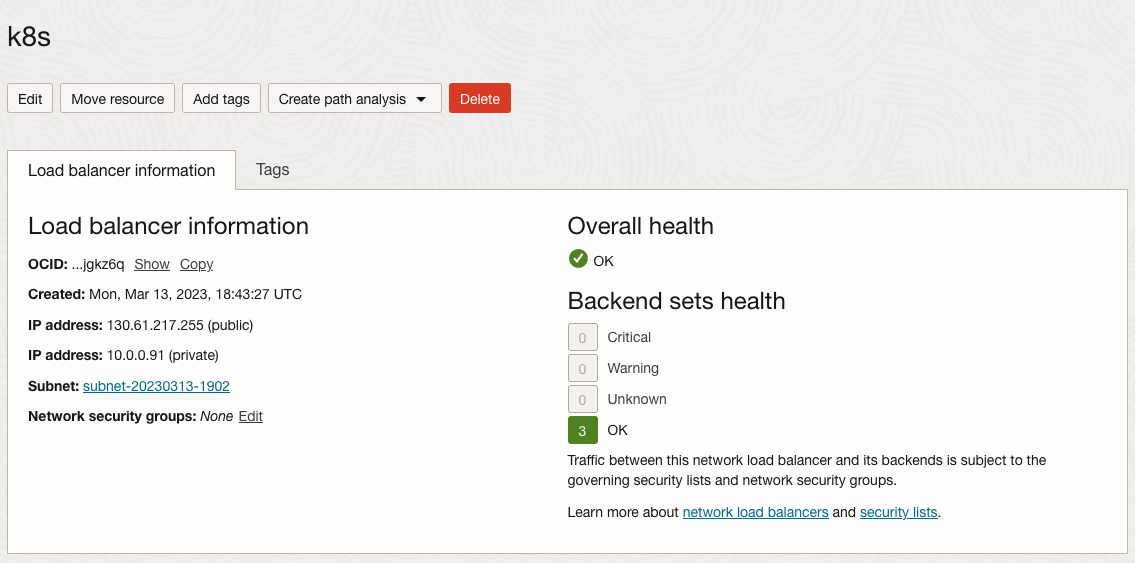
\includegraphics[width=\textwidth]{img/oci-network-load-balancer-k8s}
    \caption{Specyfikacja Network Load Balancera k8s}
    \label{fig:oci-network-load-balancer-k8s}
\end{figure}

Został skonfigurowany tak aby działał dla ruchu HTTP (port 80), HTTPS (port 443) oraz Kubernetes API (port 16443).
Dla każdego z rodzajów ruchu został utworzony Backend Set (\autoref{fig:oci-network-load-balancer-k8s-backend-sets}) oraz Listener (\autoref{fig:oci-network-load-balancer-k8s-listeners}).

\begin{figure}[H]
    \centering
    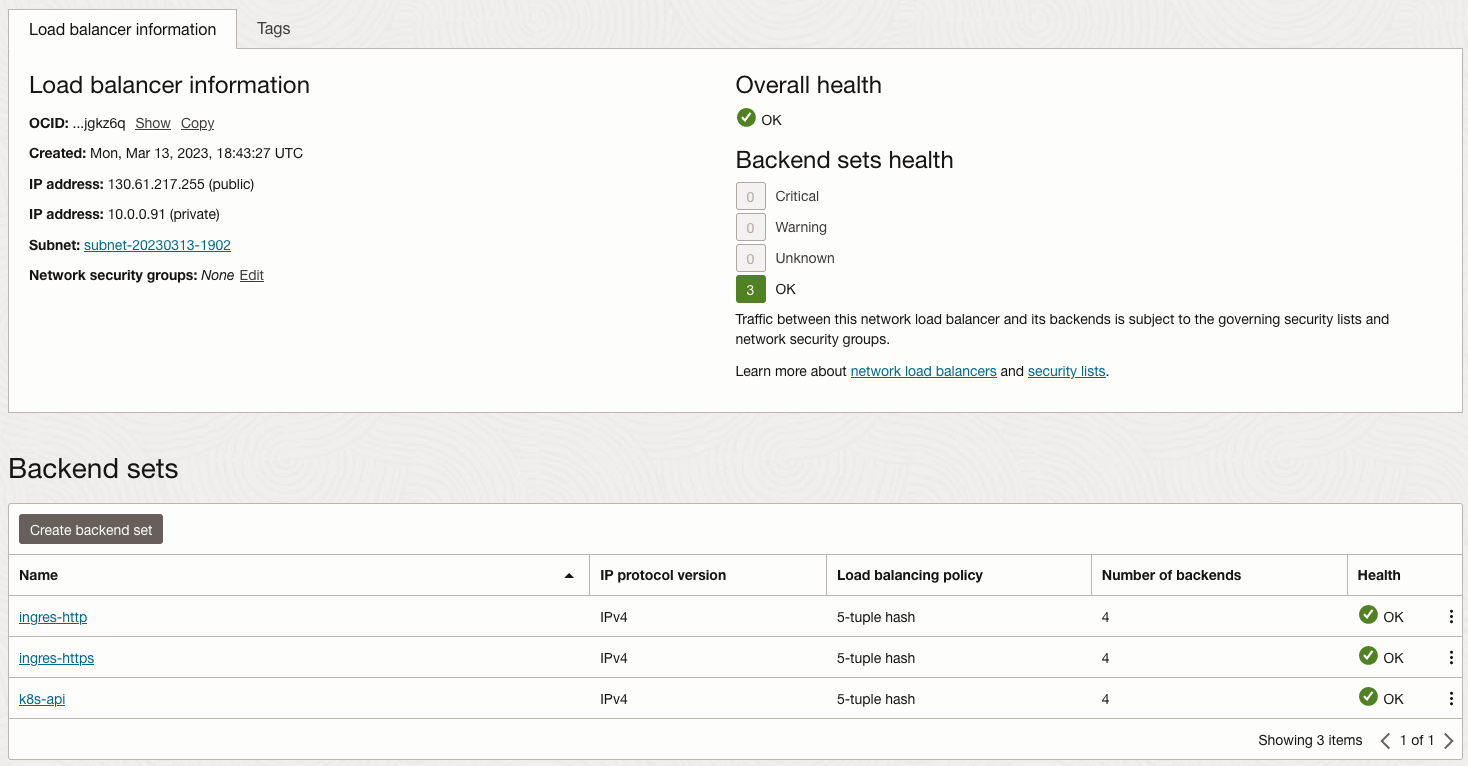
\includegraphics[width=\textwidth]{img/oci-network-load-balancer-k8s-backend-sets}
    \caption{Backend Sets stworzonego Network Load Balancera k8s}
    \label{fig:oci-network-load-balancer-k8s-backend-sets}
\end{figure}

\begin{figure}[H]
    \centering
    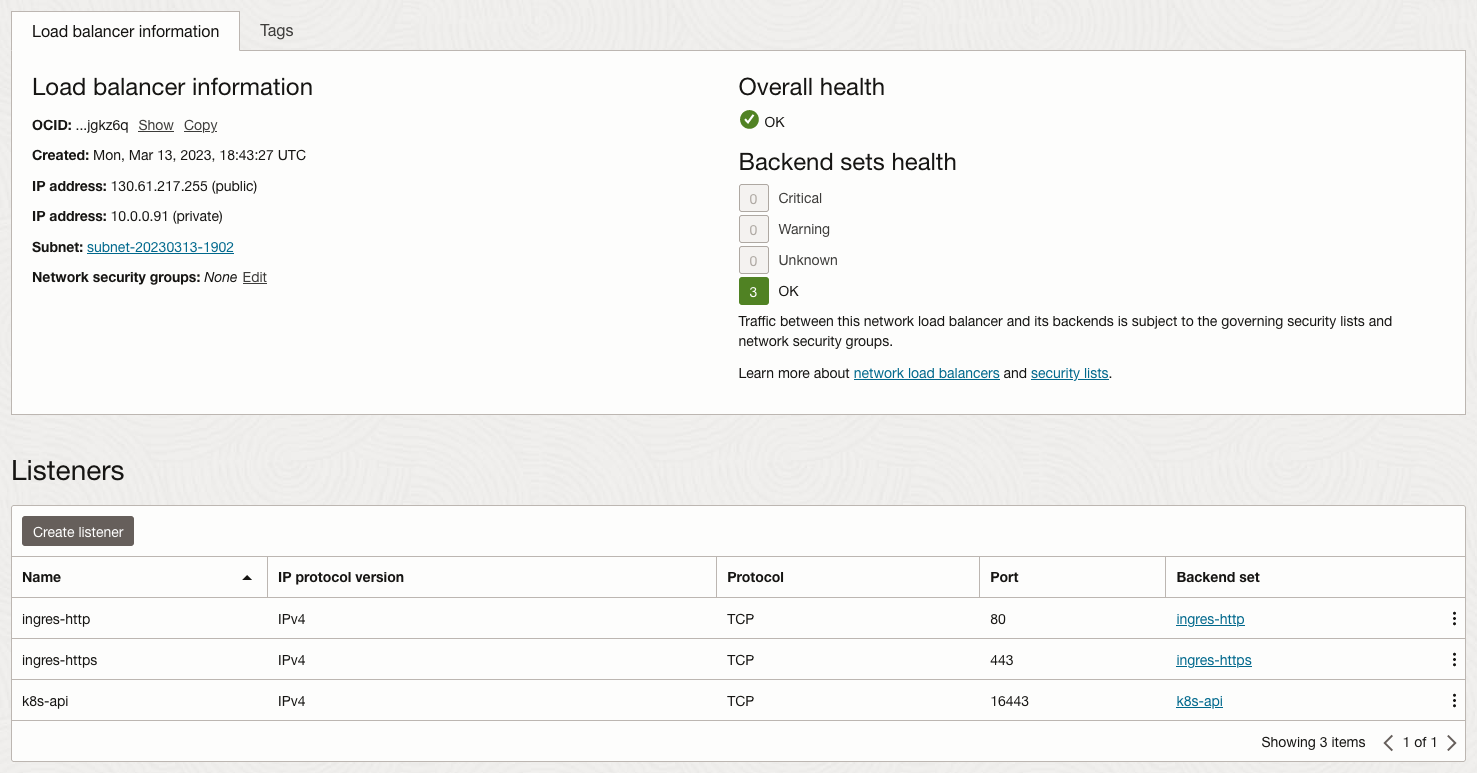
\includegraphics[width=\textwidth]{img/oci-network-load-balancer-k8s-listeners}
    \caption{Listeners stworzonego Network Load Balancera k8s}
    \label{fig:oci-network-load-balancer-k8s-listeners}
\end{figure}

Load Balancer regularnie monitoruje stan zdrowia każdego węzła za pomocą zdefiniowanego testu Health Check.
Dla pierwszych dwóch Backend Sets - \("\)ingress-http\("\) oraz \("\)ingress-https\("\) - test polega na wysłaniu zapytania z użyciem kolejno protokołu HTTP i HTTPS na ścieżkę \url{/}.
Oczekiwaną odpowiedzią serwera jest status 404.

\begin{multicols}{2}
    \begin{figure}[H]
        \centering
        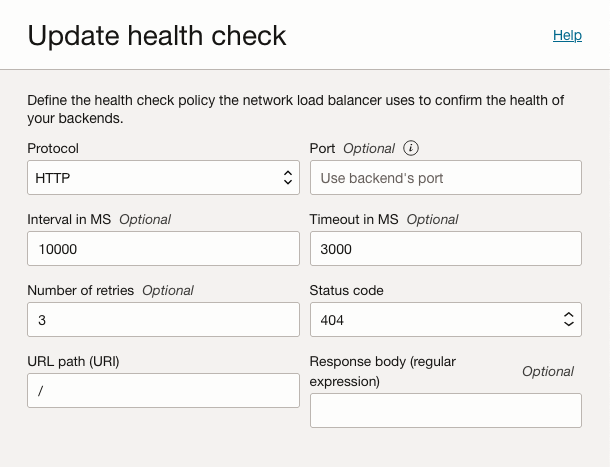
\includegraphics[width=0.5\textwidth]{img/oci-network-load-balancer-ingress-http-health-check}
        \caption{Health Check dla ingress-http}
        \label{fig:oci-network-load-balancer-ingress-http-health-check}
    \end{figure}
    \begin{figure}[H]
        \centering
        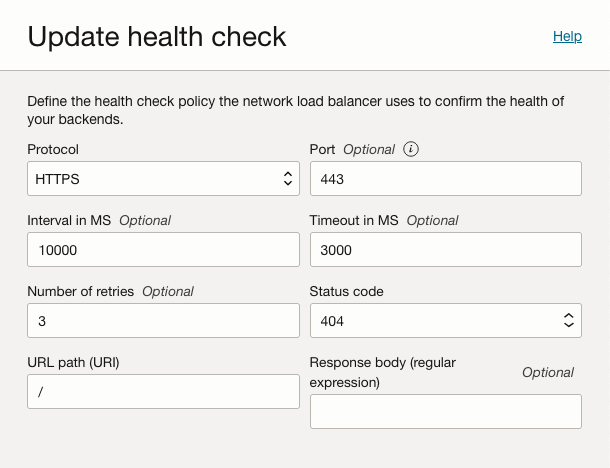
\includegraphics[width=0.5\textwidth]{img/oci-network-load-balancer-ingress-https-health-check}
        \caption{Health Check dla ingress-https}
        \label{fig:oci-network-load-balancer-ingress-https-health-check}
    \end{figure}
\end{multicols}

Natomiast dla ostatniego Backend Set k8s-api, zapytanie wysyłane jest protokołem HTTPS na port 16443 do ścieżki \url{/healthz}, gdzie oczekiwaną odpowiedzią serwera jest status 200.
\begin{figure}[H]
    \centering
    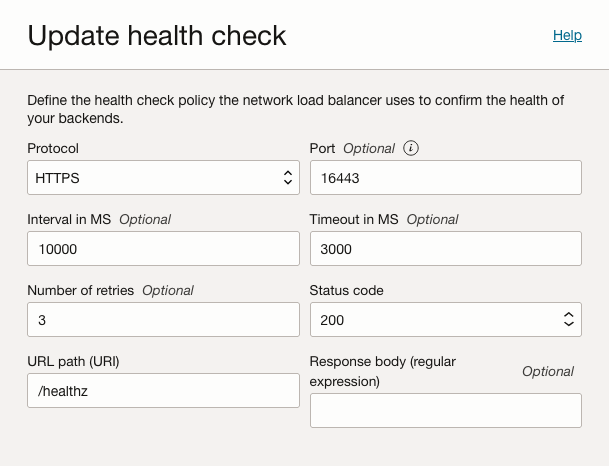
\includegraphics[width=\textwidth]{img/oci-network-load-balancer-k8s-api-health-check}
    \caption{Health Check dla k8s-api}
    \label{fig:oci-network-load-balancer-k8s-api-health-check}
\end{figure}

\subsubsection{Instalacja Kubernetes}

Kubernetes stał się obecnie niejako standardem w branży IT\@.
Na fali jego rosnącej popularności kolejne osoby oraz firmy zaczęły dostosowywać oryginalny projekt do swoich potrzeb, tym samym tworząc jego własne dystrybucje.
Chociaż wszystkie one mają wspólny fundament, będący oryginalnym Kubernetes, każda z nich wnosi unikalne funkcjonalności, narzędzia i optymalizacje.
Dla przykładu mamy takie dystrybucje Kubernetes jak Amazon Elastic Kubernetes Service (Amazon EKS), Google Kubernetes Engine (GKE) czy Azure Kubernetes Service (AKS), które zostały specjalnie dostosowane pod specyficzne środowisko chmury danego dostawcy.

\begin{samepage}
    Dla konfigurowanej platformy wybór padł na dystrybucję MicroK8s\cite{microk8s-docs-home}.
    Decydującymi czynnikami były:
    \begin{enumerate}
        \item Łatwość instalacji i uruchomienia.
        \item Fakt, że jest to lekka dystrybucja K8s, co przekłada się na mniejsze wymagania sprzętowe oraz mniejsze zużycie zasobów.
        \item Stabilność - dystrybucja jest przygotowania do produkcyjnego uruchomienia.
        \item Prostota zarządzania. MicroK8s udostępnia rozbudowany interfejs wiersza poleceń (ang. command line interface, CLI), który ułatwia konfigurację i utrzymanie środowiska.
    \end{enumerate}
\end{samepage}

MicrokK8s zostało zainstalowane na każdej z maszyn wirtualnych następującym poleceniem:
\begin{minted}{bash}
    apt update && \
        apt install docker.io -y && \
        snap install microk8s --classic --channel=1.23/stable
\end{minted}

\subsubsection{Konfiguracja certyfikatów Kubernetes API}

